\section{TSTL Tools}

The following tools are provided in the TSTL distribution on github \cite{tstl}.  Installing the TSTL module allows the compiler, called {\tt tstl} to be used at the command line.  Other tools are included in the {\tt generators} and {\tt utilities} directories of the distribution as Python scripts.

\subsection{The TSTL Compiler}

Given a harness file defined in the language discussed above, the TSTL compiler generates a stand-alone Python class that allows testing of the SUT.  This generated code does not depend on the TSTL system being installed, only on any modules the testing itself uses, and on whether code coverage is requested.  By default, the compiler produces a class supporting code coverage using the {\tt coverage.py} module, and assumes this is installed.  The TSTL compiler also allows a user to control some fine-grained coverage measures, and force a system where state-storage based backtracking is impossible to use test-replay based backtracking.

\subsection{Test Generators}

TSTL comes with a complex, highly configurable, pure random tester (supporting numerous command-line options), and simple depth-first-search and breadth-first-search based backtracking model checkers.  The included random tester provides a number of useful options, of which a subset are shown in Figure \ref{tab:rt}.  One of these, the {\tt stutter} option, is a (to our knowledge) novel idea in random testing, where any action enabled in a step has a fixed probability of being repeated.  TSTL makes implementing novel test generation methods simple, as discussed below.

\begin{figure}
{\scriptsize
\begin{itemize}
\item {\tt depth <int>}: Determines the length of generated tests.
\item {\tt timeout <int>}: Determines the maximum time spent generating tests, in seconds.
\item {\tt seed <int>}: Determines the random seed for testing.
\item {\tt maxTests <int>}: Determines the maximum number of tests to be generated.
\item {\tt stutter <float P>}: If this option is provided, the random tester will repeat any still-enabled actions with probability P.
\item {\tt running}: Produce on-the-fly, time-stamped code coverage information, for analyzing performance of testing algorithms. 
\item {\tt replayable}: Produce a log of the current test, so even it crashes Python the test can be reproduced, delta-debugged, made stand-alone, or otherwise analyzed.
\item {\tt total}: Produce a total log of all test activity, including across resets, for systems where reset is not complete (so tests across resets can be delta-debugged).
\item {\tt quickTests}:  Produce ``quick test'' files \cite{icst14}, each containing a minimal test to cover a set of branches of the SUT. 
\item {\tt normalize}: Apply additional, custom term-rewriting based simplifications of test cases that often further minimize delta-debugged test cases. 
\item {\tt generalize}: Apply generalization that elaborates each failing test with annotations showing similar tests that also fail. 
\end{itemize}
}
\caption{Some options for the TSTL random test generator.}
\label{tab:rt}
\end{figure}

TSTL can (unlike SPIN or most explicit-state model checkers) apply BFS or DFS search to applications.   The model checkers take some of the same command-line options as the random tester, but are considerably less full-featured, since exhaustive generation is applicable to fewer Python libraries (for instance, it is possible but impractical for the ArcPy implementation, due to the overhead of backtracking via replay).  TSTL also supports custom abstraction of pools:  if a pool is declared with an {\tt ABSTRACT} annotation, the function after the {\tt ABSTRACT} keyword is used to abstract all values for state-matching purposes during exhaustive exploration methods.  without support for backtracking (e.g., where Python's {\tt deepcopy} fails because some object state is handled by a Python C extension), using replay-based state storage and retrieval.

\subsection{Utilities for Test Case Manipulation}

TSTL provides the tools {\tt sandboxreducer} and {\tt standalone} for manipulating saved test cases produced by the random tester or the simple model checkers.  These were developed as part of the ArcPy testing process.  ArcPy faults tend to crash the system (this is also the reason the {\tt total} option was introduced), and thus cannot be simplified for debugging inside the test generator.   The sandbox reducer takes a testing log and, using subprocesses to handle crashes, produces delta-debugged and normalized test cases. It is also useful to report failing tests not as TSTL's internal test file format, but as standalone Python programs that cause a failure.  The {\tt standalone} utility takes a test log or a saved test case and produces a complete, stand-alone Python program that requires neither the SUT class nor TSTL.

\subsection{Visualization of Action Spaces}

\begin{figure}
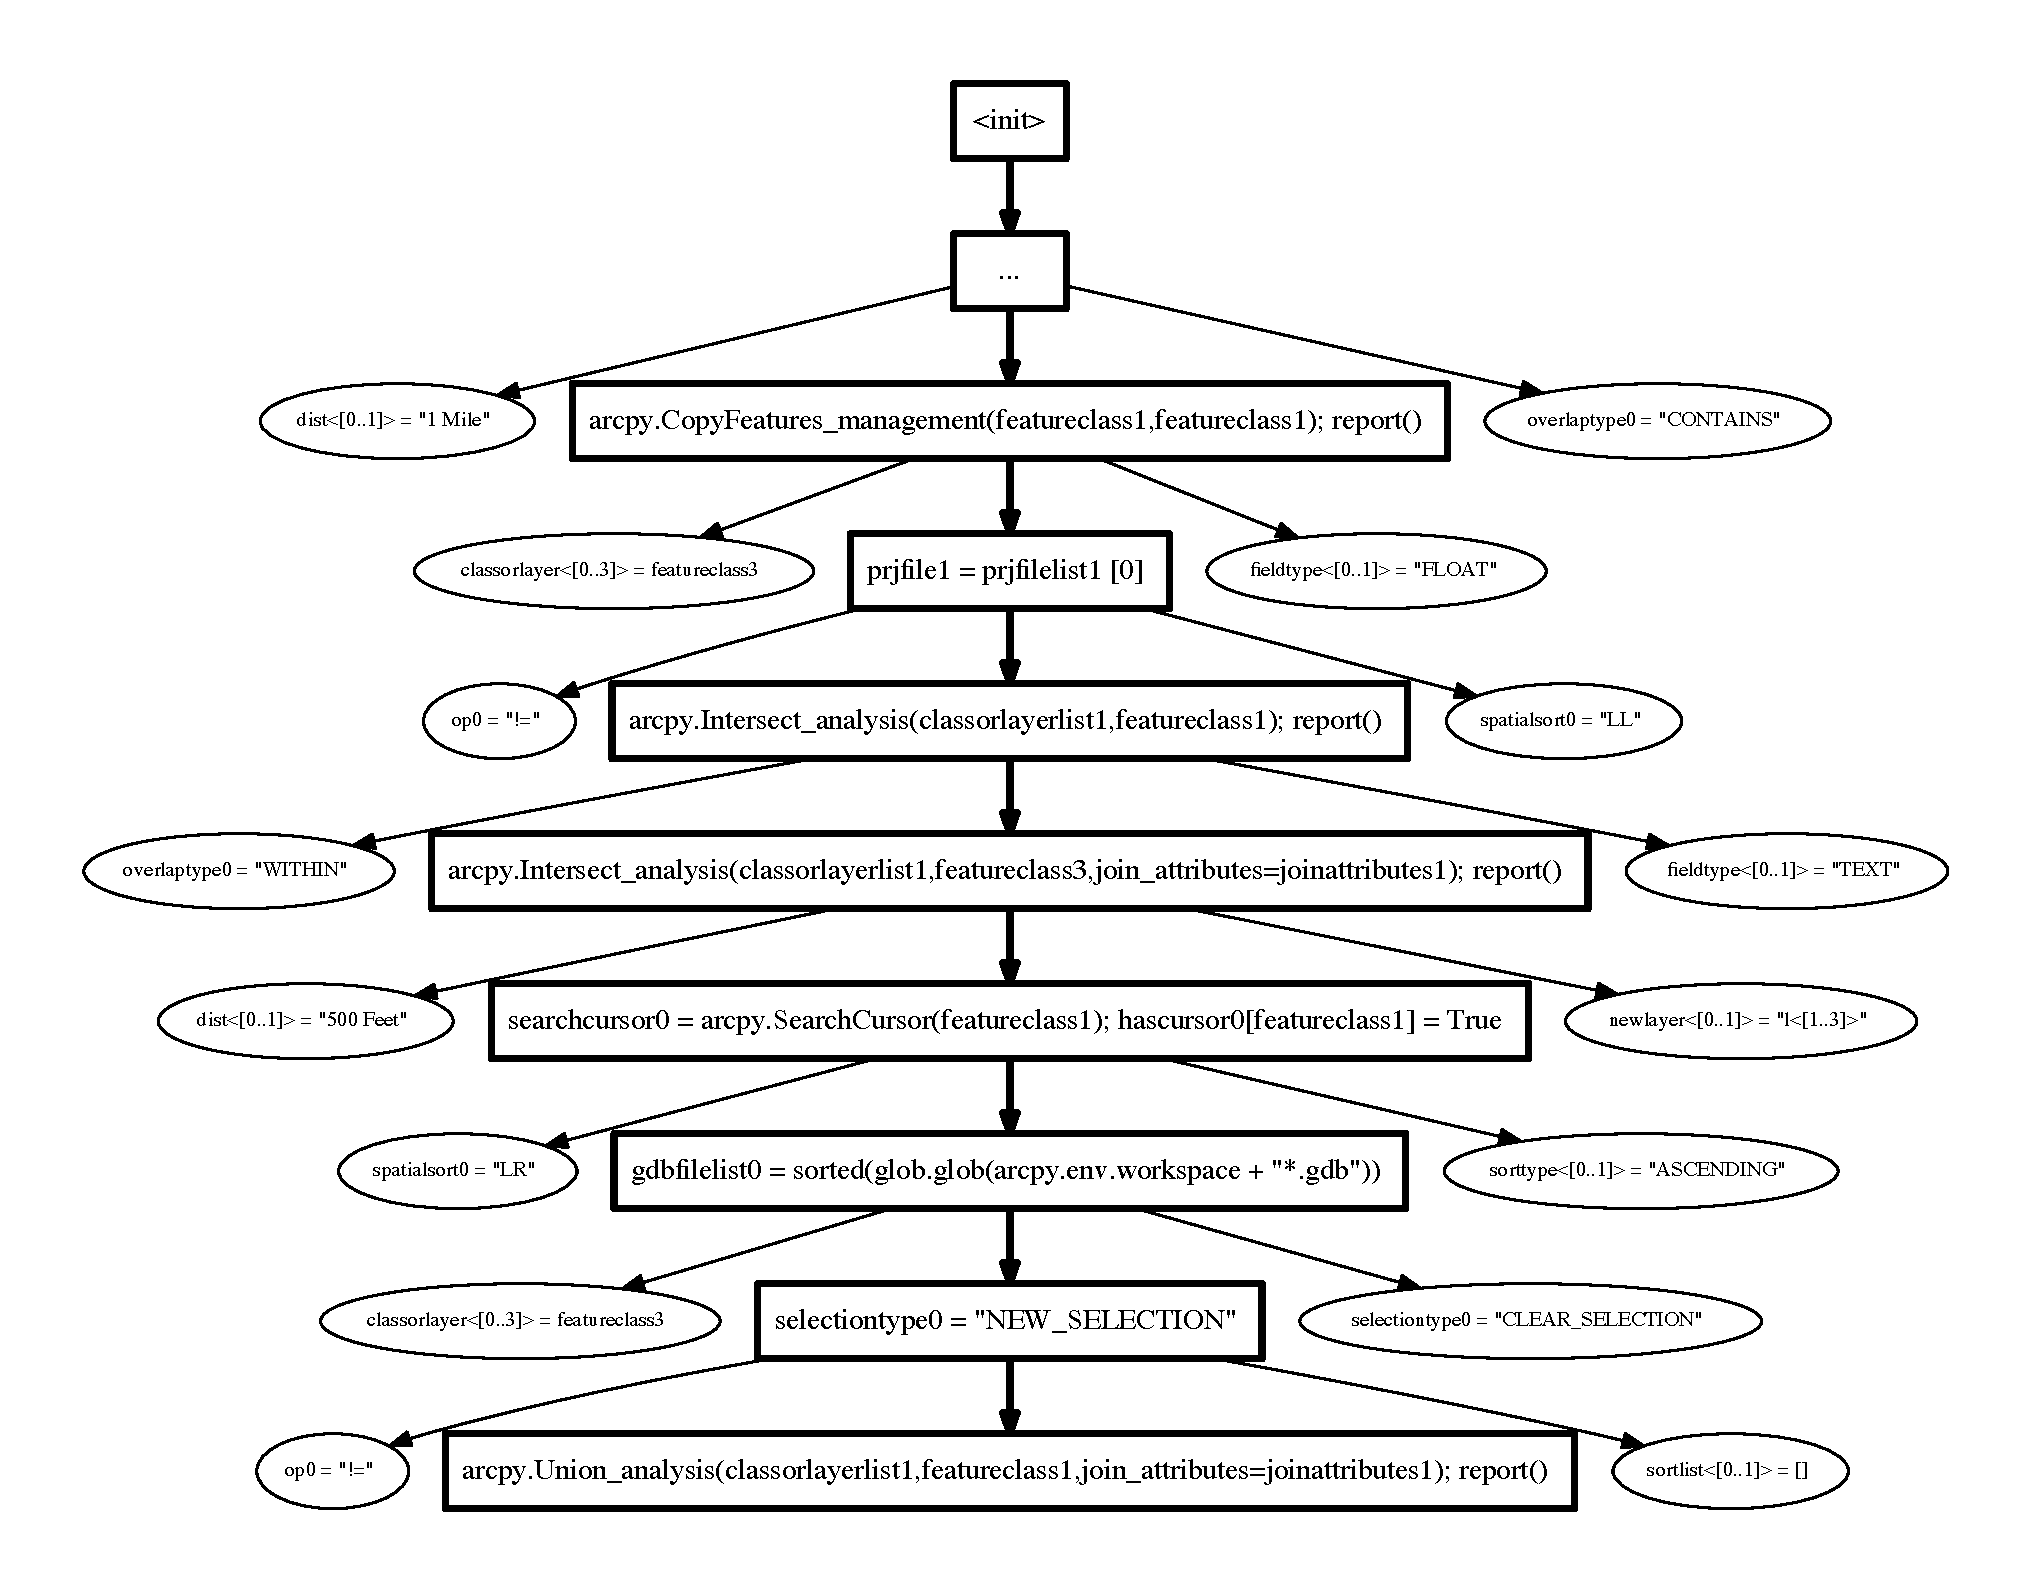
\includegraphics[width=\columnwidth]{shortgraph}
\caption{Start depth 20, depth 8, width 3 trace visualization for ArcPy testing.}
\label{fig:actions}
\end{figure}

Understanding the structure of the action graph produced by even a relatively simple TSTL harness can be difficult.  The structure is often infinite, and even in cases where there is a finite state space (perhaps introduced by abstraction) the graph is usually far too large for a convenient display.  However, we have found that a visual representation of typical trajectories through the system can be very helpful for understanding a complex test system.  The {\tt makegraph} utility takes as input a number of traces to produce, a starting depth, additional depth, and a test width.  It then produces in pdf form a number of graphs for traces like the one shown in Figure \ref{fig:actions}.  These trace graphs show, in bold, the actual action sequence chosen by a pure random tester, starting after a number of actions not shown (represented by the ``...'' node) and continuing up to the depth limit.  In addition to the actions taken, the graph also shows a random subset of additional enabled actions, with each step showing a number of actions equal to the width.  Because many actions are extremely similar, the graphing utility also summarizes actions that are the same, except for pool choice or integer constant, using the {\tt <[i..j]>} notation of TSTL.

\section{Building Your Own Tools}

Describing the full interface provided by TSTL for use in testing tools is beyond the scope of this paper.  However, examining the source code of the included testers can provide a good starting point.  Implementing new test case manipulations usually involves understanding TSTL internal structures and how tests are stored.  Implementing novel test generation algorithms can often rely on just a handful of methods, shown in Figure \ref{methods} (there are many more methods for e..g, code coverage, but this minimal set can implement many test generation algorithms).

\begin{figure}
{\scriptsize
\begin{itemize}
\item {\bf restart():}  resets the system state and aborts the current test. 
\item {\bf enabled():} returns a list of all currently enabled actions.
\item {\bf randomEnabled(random):}  given a Python random number generator object, returns a random enabled action, efficiently (avoiding unnecessary guard evaluations).
\item {\bf safely(action):} performs action (usually changing SUT state)  and returns a Boolean indicating whether the action performed raised any uncaught exceptions. 
\item {\bf check():} returns a Boolean indicating whether any properties fail for the current state.
\item {\bf error():} returns either {\tt None} (no error for the last action or {\tt check}), or a Python object representing an uncaught exception or failed property's backtrace.
\item {\bf state():} returns the current SUT state, as a set of values for all pools; for systems where state cannot be restored by pool values, or {\tt deepcopy} does not work, returns the current test to replay (can be controlled at runtime, or set as default for an SUT).
\item {\bf backtrack(state):} takes a state produced by {\tt state} and restores the system to that state; replays a test, if state-based backtracking is turned off.
\item {\bf allBranches():} returns the set of branches covered during all testing.
\item {\bf newBranches():} returns the set of branches covered during the last action executed that had not previously been covered.
\item {\bf currBranches():} returns the set of branches covered during the current test.
\end{itemize} 
}
\caption{Some core methods for testing an SUT.}
\label{methods}
\end{figure}

For example, a researcher aware of the literature showing that for many systems it is difficult to outperform random testing, due to its very low overhead \cite{ISSRE12,ISSTA12}, may consider simple modifications of random testing that do not greatly increase overhead.  One such example, with implementation, is shown in the original TSTL paper \cite{NFM15}.  We present another here.  Since the focus of this paper is on showing how to use TSTL, not novel test generation methods, we leave a complete development and statistically valid evaluation of our proposed approach to future work, but discuss briefly how to go about prototyping and evaluation using TSTL.

The idea is to perform random testing, but keep the final state of tests with unusually high coverage as potential starting points for future tests, potentially extending them far beyond the normal test length limit.  The approach is parameterized by {\tt MEMORY}, the number of ``good'' tests to store, by {\tt PEXTEND}, the probability of choosing to extend a ``good'' test rather than start a new test, and by a {\tt TIMEOUT} parameter.  Leaving out imports and other boilerplate, the entire implementation, is shown in Figure \ref{fig:keepgood}.

\begin{figure}
{\scriptsize
\begin{code}
goodTests = []
startTime = time.time()
while (time.time() - startTime <= TIMEOUT):
   if (len(goodTests) > 0) and (rgen.random() < PEXTEND):
     sut.backtrack(rgen.choice(goodTests)[1])
   else:
     sut.restart()
   for s in xrange(0,TEST\_LENGTH): 
      action = sut.randomEnabled(rgen)
      r = sut.safely(action)
      if len(sut.newBranches()) > 0:
         print time.time(),len(sut.allBranches()),'NEW BRANCHES:', sut.newBranches()
   if MEMORY > 0:
      goodTests.append((sut.currBranches(), sut.state()))
      goodTests = sorted(goodTests, reverse=True)[:MEMORY]
\end{code}
}
\caption{Implementing a very simple novel testing algorithm.}
\label{fig:keepgood}
\end{figure}

The implementation is trivial, relying only on the TSTL API and some very simple Python tools (sorting with automatic lexical ordering, time library, etc.).  We omit handling of failed tests, assuming the goal of this algorithm is simply to improve code coverage in fault-free systems for experimental evaluation.  This simple tool can be applied to any TSTL harness and will produce output showing when, in time, new branches were covered by the system.  This data can be used to produce Average-Percent-Branches-Detected (APBD) values and discovery curves \cite{issta14}. Comparison with simple random testing is easy, since setting {\tt MEMORY} to 0 gives pure memoryless random testing (alternatively, to avoid the overhead of the comparisons with 0, a dedicated version for random testing can be written).  A major threat in most comparisons of testing algorithms is that different underlying infrastructure for different methods may end up outweighing even moderately sized effects due to the underlying algorithms.  With TSTL, fair comparisons are much easier, since the TSTL interface does most of the computational work that is common to multiple algorithms, with the same overhead.  Evaluating an algorithm can be as simple as finding a large number of suitable programs without failures (or where failures don't make coverage values invalid) and performing enough trials to establish statistical validity for comparisons with APBD values for known algorithms.  Evaluation in terms of discovered faults or time-until-discovery of a fault is nearly as simple.  This algorithm is of some interest, in that while it requires backtracking, the frequency of backtracking is low enough to be potentially applicable even to systems like ArcPy where backtracking is only possible via expensive test replay.  While a mature version of this method would require many SUTs and experiments, as well as investigation of suitable values for {\tt MEMORY} and {\tt PEXTEND}, Figure \ref{fig:compare} shows that average branch discovery curves for ArcPy can sometimes be improved, even using the  arbitrarily chosen parameters of a size 5 memory and a 20\% probability of using a ``good'' test as a starting point.  The simplicity of the Python implementation makes performing automatic experiments with different parameters and test lengths trivial.  Experiments can also take advantage of Python libraries for automatic statistical analysis and plotting of results.

\begin{figure}
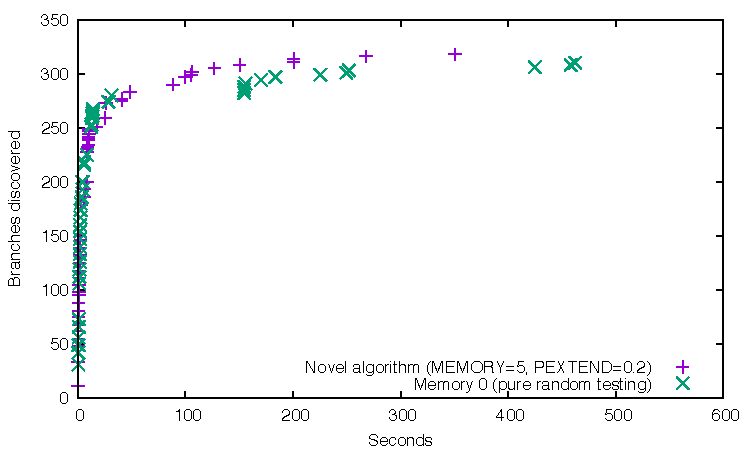
\includegraphics[width=\columnwidth]{memory}
\caption{Comparing value for a 10 minute runs using MEMORY = 5, PEXTEND = 0.2 and pure random testing.}
\label{fig:compare}
\end{figure}